\documentclass[a4paper]{article}

\usepackage[english, ngerman]{babel}
\usepackage[T1]{fontenc}
\usepackage[utf8]{inputenc}
\usepackage{graphicx}
\usepackage{hyperref}
\usepackage{filecontents}
\usepackage{multirow}
\usepackage{booktabs}
\usepackage[backend=biber,style=numeric, autocite=plain,sorting=none]{biblatex}
\usepackage{hyperref}
\usepackage[raggedright]{titlesec}
\usepackage{enumitem}
\usepackage{doi}
\usepackage{url}
\usepackage[automark,headsepline]{scrlayer-scrpage}
\usepackage{color}
\usepackage{xcolor}
\usepackage{sectsty}
\usepackage{titlecaps}
\usepackage{titlesec}
\usepackage{palatino}
\usepackage[defaultsans]{droidsans}

\definecolor{purple}{RGB}{148, 82, 165}
\newcommand{\todo}[1]{{\color{purple}{#1}}}

\hypersetup{colorlinks=true,citecolor=black,filecolor=black,linkcolor=black,urlcolor=black}

\renewcommand\thesection{\Roman{section}}
\renewcommand\thesubsection{\arabic{subsection}}


%\titleformat*{\section}{\normalfont\Large\bfseries\epigrafica}
%\titleformat*{\subsection}{\normalfont\large\bfseries\epigrafica}
%\titleformat{\subsubsection}[hang]{\normalfont\Large\bfseries\epigrafica}{\thesubsubsection}{1em}{}%TODO


\titleformat{\paragraph}[hang]{\normalfont\normalsize\bfseries}{\theparagraph}{1em}{}
\titlespacing*{\paragraph}{0pt}{3.25ex plus 1ex minus .2ex}{0.5em}
%Formatierung des Paragraphen, sodass eine neue Zeile beginnt




%\titleformat*{\subparagraph}{\bfseries\itshape}
%\titlespacing*{\subparagraph}{0pt}{3.25ex plus 1ex minus .2ex}{0.5em}

% package for bibliography
%\usepackage[numbers]{natbib}

%\bibliographystyle{unsrtnat}

\addbibresource{Referenzen.bib}


\pagestyle{scrheadings}
\ihead[]{Dark Patterns}
\ohead[]{\today}%bla
\cfoot[]{\pagemark}

\setcounter{secnumdepth}{4}
%section depth (value steht fuer Stellen); bei 4 werden die Paragraphen durchnummeriert
\setcounter{tocdepth}{3}
%table of content depth




\begin{document}
	\title{
	\begin{figure}[!ht]
		% \flushleft
			%\includegraphics[width=0.26\textwidth]{img/THlogoheader.pdf}
	\end{figure}
	\vspace{1cm}
	\Huge Dark Patterns
	}
	
	\vspace{1cm}

	

	\author{\Large \href{mailto:natalie.tork_alinaghipour@smail.th-koeln.de}{Natalie Tork Alinaghipour} 
	\vspace{1cm}}
	
	% name of the course and module
	\date{
	\large Praxisprojekt Wintersemester 2020/2021 \\ 
	\vspace{0.8cm}
	\large Betreuer: Prof. Gerhard Hartmann \\
	\vspace{1cm}
	\today
	}

	\maketitle
	\setlength{\parindent}{0pt}

\vspace{2cm}
	\newpage
	\tableofcontents
	\newpage
	
\section{Einleitung} 
\label{sec:einleitung}

\subsectionfont{\MakeUppercase}
\subsection{Problemfeld und Kontext}
\label{sub:problemfeld_und_kontext}
Bei der Gestaltung von digitalen Systemen spielt die User Experience (UX) eine wichtige Rolle für Online-Marketing und -Vertrieb, da sie maßgeblich zum Erfolg eines Unternehmens beiträgt. UX Design basiert unter anderem auf psychologischen und verhaltensökonomischen Erkenntnissen und hat langfristig zum Ziel, die Erfahrung des Nutzers während der Interaktion eines Produkts zu verbessern. Allerdings können diese Methoden auch dazu missbraucht werden, die menschliche Wahrnehmung und Verhaltensweisen zu beeinflussen, um wirtschaftlich davon zu profitieren. Nutzer können so zu nicht intendierten Taten verleitet und infolgedessen benachteiligen werden. Dies zu bemerken ist für viele schwierig, da der Zweck nicht transparent gemacht wird.
Diese Taktiken werden als \textit{Dark Patterns} bezeichnet und werden bereits ethisch erforscht. Heutzutage findet diese Art von manipulativem Design in vielen verschiedenen Bereichen Anwendung, wie in Desktop-, Web- oder Mobilen Applikationen, sowie in Videospielen, Proxemischer Interaktion\footnote{\label{foot:1} Proxemische Interaktion bedeutet die Verbundenheit und Kommunikation zwischen Geräten und zwischen Mensch und Maschine, sobald diese sich in unmittelbarer Nähe zueinander befinden} und Künstlicher Intelligenz. 


\subsection{Ist-Zustand}
\label{sub:ist-zustand}
Der Begriff \textit{Dark Patterns} wurde Harry Brignull\footnote{\label{foot:2} Als UX-Experte und Doktor der Kognitionswissenschaften setzt er sich noch heute aktiv gegen diese Methoden in digitalen Produkten ein und agiert als Sachverständiger in dem Bereich. Zudem führt er zusammen mit Alexander Darlington (UX Researcher und Forscher im Ethischen Design die Webseite darkpatterns.org, auf der Brignull die von ihm definierte Taxonomie von Dark Patterns beschreibt, und macht auf dem dazugehörigen Twitter-Account öffentlich auf das Thema aufmerksam \cite{brignull3}\cite{brignull4}.} geprägt, als er im Jahr 2010 einen Blog-Beitrag veröffentlichte \cite{brignull1} und kurze Zeit später einen Vortrag auf der UX Brighton Conference hielt. Inzwischen wurden bereits einige Paper über das Thema verfasst, die verschiedene Nutzungskontexte beschreiben. Da demnach viele unterschiedliche Technologien Dark Patterns enthalten, ist der Themenbereich recht unübersichtlich und komplex, wodurch eine ausführliche Recherche notwendig ist.

\subsection{Ziel und Lösungsansatz}
\label{sub:ziel_und_loesungsansatz}
Das Ziel soll es sein, eine Übersicht in das Themenkomplex Dark Patterns zu bringen, indem diese nach Systemen strukturiert werden. Es soll analysiert werden, welche Dark Patterns zu den jeweiligen Nutzungskontexten existieren. Ebenso gilt es herauszufinden, welche Zielgruppe von diesen Methoden betroffen sind und wer die Stakeholder sind. 

\newpage

\subsection{Motivation}
\label{motivation}
Das Thema hat eine hohe gesellschaftliche Relevanz, da heutzutage das Internet für die meisten Menschen in das Leben integriert ist. Alltägliche Aufgaben können dadurch einfacher und schneller bewältigt werden. Jedoch kann die Tatsache, dass viele auf eine gute Usability angewiesen sind, ausgenutzt werden und demnach stellt dies ein mögliches Risiko dar. 
Zudem hat die Datenschutz-Grundverordnung dazu geführt, dass die Bedingungen der Nutzung bestimmter Dienste zu umfangreich und zu kompliziert formuliert sind, sodass das Lesen unnötig erschwert oder gar unmöglich gemacht wird. Dies hat zur Folge, dass Nutzer wegen Zeit- und Alternativenmangel diesen Bedingungen zustimmen, ohne diese vollständig zu lesen.  
Aus den oben genannten Gründen weist das Thema auch eine hohe politische Relevanz auf, da es von großer Notwendigkeit ist, Verbraucher durch sinnvolle Maßnahmen vor alldem zu schützen und sie auf Dark Patterns aufmerksam zu machen.

\newpage

\section{Hintergrund}
\label{sec:hintergrund}

\subsection{Über Dark Patterns} 
\label{sub:die_hintergruende_der_dark_patterns}
Der Ausdruck Dark Patterns, auch als  \glqq Deceptive Design\grqq{} oder \glqq Unethical Design\grqq{} bezeichnet, stammt von Harry Brignull, welches er wie folgt definiert:
\begin{quote}
\glqq \textit{A user interface that has been carefully crafted to trick users into doing things… they are not mistakes, they are carefully crafted with a solid understanding of human psychology, and they do not have the user's interest in mind.}\grqq{}
\end{quote}
Demnach werden solche Benutzeroberflächen strategisch mit manipulativen Methoden gestaltet auf Basis von menschlichen Denk-, Wahrnehmungs- und Verhaltensmustern, sodass Einflussnahme auf diese genommen werden kann. Dies kann negative Konsequenzen für den Nutzer nach sich ziehen, wenn sie zur Ausführung von unbeabsichtigten Aktionen verleitet werden.\newline
Heutzutage sind Apps und Online-Dienste fester Bestandteil des alltäglichen Lebens. Dabei ist die Informationsflut unvermeidbar, in der Nutzer ständig vor Entscheidungen gestellt werden im Bezug auf Vertragsbedingungen und Einwilligung der Verarbeitung persönlicher Daten. Es fehlt die Zeit, sich zu informieren und gründlich über Entscheidungen nachzudenken, und dabei nehmen Nutzer eine Begegnung mit Dark Patterns oftmals nicht wahr, da sie gut versteckt sind. Manche sorgen lediglich für Frust und Ärger, hinter anderen steckt allerdings eine gezielte Täuschungsabsicht, die beispielsweise zu finanziellem Verlust, zu zwanghaftem oder Suchtverhalten führt, sowie die Nutzer dazu bringt, persönliche Informationen preiszugeben \cite{mathur}. Besonders bei unerfahrenen Nutzer, wie Kindern, Jugendlichen, Senioren, Menschen mit Behinderung und bildungsfernen Gruppen, kann dies Schaden anrichten \cite{tab}. \newline\newline
Bei der Anwendung von Dark Patterns auf digitale Produkte hat sich vor allem A/B-Testing\footnote{\label{foot:1}A/B-Testing ist eine UX Research Methode, bei der Testpersonen zwei Varianten eines Prototypen gezeigt werden und daraufhin untersucht wird, welche Variante effektiver ist.} als ein hilfreiches Werkzeug für die Kundengewinnung, Umsatzsteigerung und Maximierung der Nutzungsdauer erwiesen, unter anderem im Rahmen von Neuromarketing \cite{snv}\cite{narayanan}\cite{tab}. Doch nicht nur im Onlinehandel mit Waren oder Dienstleistungen sind Dark Patterns zu finden. Darüber hinaus werden sie auch eingesetzt unter anderem in Online-Diensten, wie E-Mail-Dienste, Suchmaschinen, Download- und Streaming-Anbietern, sowie in Social Media Plattformen \cite{fastcompany}, Betriebssystemen von Computern und Smartphones, in Buchungsportalen \cite{swr}, Smart-TVs \cite{bundeskartellamt} und Games. Ebenso werden unethische Design-Methoden bereits in neuartigen Technologien erforscht, etwa in der Robotik oder in proxemischen Interaktions-Systemen.  

\subsection{Allgemeine Dark Patterns Kategorien}
\label{sub:dark_patterns_kategorien}
Brignulls 12 Typen von Dark Patterns werden von Gray et al. in Kategorien eingeteilt, die die Strategien und Motivation dahinter zusammenfasst \cite{gray}. 
Im Folgenden wird erläutert, was unter den einzelnen Kategorien zu verstehen ist und wie die Taxonomie von Brignull in diese einzuordnen ist. Diese Praktiken finden allgemein in der Gestaltung von digtalen Benutzeroberflächen Anwendung.

\subsubsection{Nagging}
\label{sssec:nagging}
Während der Interaktion mit dem System wird der Nutzer ein- oder mehrmals entgegen seiner Erwartung umgeleitet und bei der Aufgabenerledigung unterbrochen. Dabei hat die Unterbrechung für den Nutzer keine Relevanz. Diese treten meist in den folgenden Formen auf:
\begin{enumerate}[label=\arabic*)]
	\item{Pop-Ups, die den Zugriff auf das Interface sperren,}
	\item{Audionotizen, die zur Ablenkung führen,}
	\item{andere Formen von Aktionen, die den Nutzer von der Erledigung seiner Aufgaben ablenken.}
\end{enumerate}

\subsubsection{Obstruction} 
\label{sssec:obstruction}
Die Erledigung der Aufgaben wird so erschwert, dass der Nutzer davon abgebracht wird. Ein mögliches Vorkommnis ist, dass der Nutzer in dem Moment, wo er auf die Barriere stößt, über die Beschränkung der nutzbaren Funktionen benachrichtigt wird. Der Nutzer muss diese Funktionen also erst freischalten.	

\paragraph{Roach Motel (Brignull)} 
\label{para:roach_motel}
Führt den Nutzer auf einen langen Pfad und ruft gleichzeitig eine Disorientierung durch unklare Formulierungen hervor. Der Nutzer gerät hier leicht in eine Situation und kommt nur schwer aus dieser Lage heraus. Dies geschieht beim Abonnieren eines Services oder der Registrierung bei einem Service, indem es dem Nutzer schwer oder sogar unmöglich gemacht wird, diesen Service wieder abzubestellen oder das Konto zu löschen.

\paragraph{Price Comparison Prevention (Brignull)} 
\label{para:price_comparison_prevention}
Hindert den Nutzer daran, Preise von Produkten und Dienstleistungen zu vergleichen. Dies kann zum Beispiel der Fall sein, wenn es dem Nutzer nicht möglich ist, Produktinformationen zu kopieren, um damit Suchanfragen stellen zu können.
% Kommentar von Dome: Außerdem: Andere Dinge zum Kauf hinzufügen. Also "Sets" anbieten. Bsp: Kaufst x, kriegst aber y dazu. Bei anderem Anbieter x aber z zusätzlich.

\paragraph{Intermediate Currency (Gray et al.)} 
\label{para:intermediate_currency}
Der Nutzer wird gezwungen, echtes Geld in eine virtuelle Währung zu investieren, damit er Käufe tätigen kann. Oft kommt dies in Apps vor, die In-App Käufe anbieten.

\subsubsection{Sneaking}
\label{sssec:sneaking}
Relevante Informationen werden vor dem Nutzer versteckt oder verschleiert, oder die Anzeige der Information wird verzögert. Ziel ist es, den Nutzer dazu zu führen, eine Aktion auszuführen, die in der Regel nicht in seinem Interesse ist, wenn er Kenntnis davon hätte. Dazu zählen versteckte Kosten oder unerwünschte Effekte durch die Ausführung einer bestimmten Aktion.

\paragraph{Forced Continuity (Brignull)}
\label{para:forced_continuity}
Wenn ein Nutzer eine Frist versäumt, soll dies ausgenutzt werden. Oft wird der Nutzer hier zur Kasse gebeten werden, wenn ein Service automatisch erneuert wird, weil dieser nicht rechtzeitig vor Ablauf einer Probezeit gekündigt wurde.

\paragraph{Hidden Costs (Brignull)} 
\label{para:hidden_costs}
Versteckte Kosten werden erst später offenbart, nachdem ein potentieller Kunde mit einem besonderen Angebot angelockt wurde. Wird dieser beispielsweise kurz vor dem Abschluss eines Bestellvorgangs darauf hingewiesen, dass das Angebot zeitlich begrenzt ist oder diverse Kosten, Steuern oder hohe Liefergebühren anfallen, so kann das auf dieses Dark Pattern hinweisen. 

\paragraph{Sneak into Basket (Brignull)}
\label{para:sneak_into_basket}
Dem Nutzer wird ohne sein Wissen automatisch ein Artikel in den Warenkorb gelegt, was unbemerkt bleiben kann, wenn der Nutzer seine Einkaufsliste vor der Bestellung nicht überprüft. Oft basieren solche Artikel angeblich auf einer Empfehlung für den Kunden.

\paragraph{Bait and Switch (Brignull)}
\label{para:bait_and_switch}
Gewohnte Interaktionselemente einer Applikation führen zu einem unerwarteten und unerwünschten Ergebnis. 
Für Aufsehen sorgte beispielsweise Microsoft im Jahr 2016, als Nutzer von älteren Windows-Versionen dazu gedrängt wurden, das Betriebssystem auf Windows 10 zu aktualisieren \cite{thurrott}. Ein Schließen der Meldung durch den entsprechenden Button führte zwar zum Schließen des Fensters, allerdings war den Nutzern nicht bewusst, dass sie dabei gegen ein Upgrade auf Windows 10 keinen Widerspruch eingelegt haben. Daraufhin wurde bei diesen Nutzern zu einem von Windows festgelegten Zeitpunkt das Upgrade durchgeführt. 
%Bild von Windows 10 Upgrade einfügen?

\subsubsection{Interface Interference}
\label{sssec:interface_interference}
Sobald bestimmte Aktionen, die überdeckt werden von anderen Aktionen, den Nutzer bei der Erledigung seiner Aufgaben stören oder die Sichtbarkeit von Aktionen oder Informationen beschränken, spricht man von Interface Interference. 
Gray \cite{gray} unterscheidet dabei zwischen \textit{Hidden Information}, \textit{Preselection} und \textit{Aesthetic Manipulation}. 

\paragraph{Hidden Information}
\label{para:hidden_information}
Sorgt dafür, dass wichtige Informationen nur schwer auffindbar und lesbar sind. Demnach bekommt der Nutzer das Gefühl vermittelt, als seien die Informationen für ihn nicht von Bedeutung. Oft sind diese dargestellt als Optionen oder als Kleingedrucktes, verblasster Text oder in Form von schwer verständlichen Geschäftsbedingungen.

\paragraph{Preselection}
\label{para:preselection}
Eine Option in einem Dialog ist von Anfang an ausgewählt, noch bevor der Nutzer eine eigene Auswahl getroffen hat. Meistens entspricht die Auswahl nicht dem Interesse oder der Absicht des Nutzers, sofern er keine Anpassungen vornimmt. Oft geht er in dem Fall dennoch davon aus, dass die Vorauswahl im besten Interesse des Nutzers ist. 
 
\paragraph{Aesthetic Manipulation (Gray et al.)}
\label{para:aesthetic_manipulation}
Die Form der Benutzeroberfläche wird so gestaltet, dass die Aufmerksamkeit des Nutzers auf etwas anderes gelenkt oder dass er von etwas anderem überzeugt wird. Brignull hat dieses Dark Pattern als \glqq Misdirection\grqq{} bezeichnet. 
Darunter fallen die Dark Patterns \textit{Toying with Emotions}, \textit{False Hierarchy}, \textit{Disguised Ad} und \textit{Trick Question}.

\subparagraph{Toying with Emotions (Gray et al.)} 
\label{subpara:toying_with_emotions}
setzt Elemente wie Farben, Sprache oder Schreibstil gezielt dafür ein, Emotionen hervorzurufen, um den Nutzer dazu zu bringen, eine bestimmte Aktion auszuführen. Hier kommen unter anderem niedliche beziehungsweise furchteinflößende Bilder, oder verlockende oder Angst machende Formulierungen zum Einsatz. Zum Beispiel kann es sich bei einem Angebot einer zeitnahen Lieferung nur um eine zeitlich begrenzte Garantie handeln, was den Nutzer unter Druck setzen kann, seinen Einkauf zügig abzuschließen. Nachforschungen von Gray zeigen allerdings, dass der Timer oft neugestartet wird, nachdem die Zeit um ist. 

\subparagraph{False Hierarchy (Gray et al.)}
\label{subpara:false_hierarchy}
erschwert dem Nutzer während eines Dialogs die Interaktion mit bestimmten Optionen oder bestimmte Optionen werden visuell anders dargestellt und vom Nutzer kaum wahrgenommen. So kann der Nutzer davon ausgehen, dass seine Auswahlmöglichkeiten beschränkt sind oder dass eine bestimmte Option für den Nutzer die bessere ist. Ein Beispiel hierfür ist die Installation von manchen Desktop-Anwendungen, bei der zu Beginn die Optionen einer (empfohlenen) Express-Installation und einer erweiterten, jedoch ausgegrauten Installation aufgelistet werden.

\subparagraph{Disguised Ad (Brignull)}
\label{subpara:disguised_ad}
versteckt eine Werbung hinter einem Navigationselement oder einem Inhalt, die nicht klar als solche gekennzeichnet ist und den Nutzer anlocken soll.
Dies kann ein interaktives Spiel, ein Download-Button oder ein anderes hervorstechendes Interaktionselement sein, die den Nutzer dann auf eine andere Seite umleitet.

\subparagraph{Trick Question (Brignull)}
\label{subpara:trick_question}
verwendet eine Frage, die doppelte Negation oder missverständliche Formulierungen enthält. Liest der Nutzer sich die Frage nicht gründlich durch, macht die Frage nur den Anschein, als wäre sie das, was der Nutzer erwartet. Mit diesem Trick wird der Nutzer dazu gebracht, mit seiner Auswahl eine Zustimmung zu geben, die nicht in seinem Interesse ist. 

\subsubsection{Forced Action}
\label{sssec:forced_action}
Der Nutzer muss eine Aktion ausführen, um (weiterhin) Zugang zu bestimmten Funktionen zu bekommen. Oft ist dies verbunden mit einem Vorgang, der nur dann abgeschlossen werden kann. Die obligatorische Aktion kann auch verschleiert werden als etwas, von dem der Nutzer angeblich profitieren würde. 
Als Beispiel gibt Gray et al. \cite{gray} Windows 10 an, das den Nutzer zwingt, beim Herunterfahren oder Neustarten des Rechners ein Update durchzuführen.  

\paragraph{Social Pyramid (Gray et al.)}
\label{para:social_pyramid}
Ein Service kann erst dann (vollumpfänglich) genutzt werden, wenn der Nutzer andere eingeladen hat. Dies kommt oft bei sozialen Anwendungen oder Online-Games vor. 

Brignulls \textit{Friend Spam} steht mit diesem Dark Patterns im Zusammenhang. Hierbei wird der Nutzer nach einer Zugriffsberechtigung für sein E-Mail Konto oder sein Konto auf einem Sozialen Netzwerk gefragt, unter dem Vorwand, ihm einen Vorteil zu verschaffen (wie zum Beispiel das Finden von Freunden zur Erweiterung seines Netzwerks bei diesem Service). Allerdings können die Kontaktdaten missbraucht werden, um im Namen des Nutzers Einladungen zu versenden, ohne dass der Nutzer davon Kenntnis hat.
Ein bekannt gewordenes Beispiel dafür war LinkedIn, die eine zeitlang von ebendieser Methode Gebrauch gemacht haben, bis sie im Jahr 2015 ein Gerichtsverfahren verloren und diese Methode daraufhin in Kalifornien als illegal erklärt wurde \cite{brignull5}.   

\paragraph{Privacy Zuckering (Brignull)}
\label{para:privacy_zuckering}
Der Nutzer wird dazu gebracht, mehr persönliche Informationen als gewollt oder notwendig preiszugeben. Diese Informationen werden dann oft an Dritte verkauft. Erst bei Durchsehen der Geschäftsbedingungen oder der Datenschutzerklärung wird dies dem Nutzer bewusst.

\paragraph{Gamification (Gray et al.)}
\label{para:gamification}
Der Nutzer wird zur wiederholten Nutzung des Services gezwungen, damit er mit bestimmten Funktionen des Services belohnt wird. Solange kann er den Service nicht im vollen Umfang benutzen. 

\newpage

\section{Nutzungskontexte von Dark Patterns} % (fold)
\label{sec:nutzungskontexte_von_dark_patterns}
Dark Patterns sind inzwischen gut erforscht, und Forschungsteams aus aller Welt verdeutlichen die Relevanz und Risiken für unterschiedliche Nutzungskontexte. Laut Gray et al. existieren verschiedene Dark Patterns Strategien, auf dessen Basis in einem weiteren Paper über 1.200 Online-Shops gefunden werden konnten, die Dark Patterns enthalten \cite{gray}\cite{mathur}. In einer weiteren Studie stellte sich heraus, dass mehr als 95\% der beliebtesten Android Applikationen Dark Patterns verwenden und konnten nachweisen, dass diese Methoden tatsächlich in der Lage dazu sind, Nutzerverhalten zu manipulieren \cite{geronimo}. Auch in Games konnten solche Strategien verschiedenen, Game-spezifischen Kategorien zugeordnet werden \cite{zagal}. Ein weiteres Risiko stellen \textit{Privacy Dark Patterns} dar, durch die Nutzer dazu gebracht werden, ihre persönlichen Daten preiszugeben, damit diese von einem Dienstleister gesammelt, gelagert und verarbeitet werden können, ohne dass eine bewusste Zustimmung gegeben wurde \cite{boesch}. 

Doch Dark Patterns beschränken sich nicht nur auf Benutzeroberflächen: auch Künstliche Intelligenz hat das Potential, für solche Zwecke missbraucht zu werden. Dazu wurde
der Effekt von \glqq Cute Robots\grqq{} auf die Preisgabe von emotionalen Daten der Nutzer analysiert \cite{lacey}. Für Geräte der Proxemischen Interaktion wurde ebenfalls, teilweise anhand von aktuellen und vergangenen Beispielen, Dark Patterns festgelegt und Prognosen angestellt.

Im Folgenden werden verschiedene Nutzungskontexte aufgeführt, in denen Dark Patterns vorkommen. Zum Teil sind die erläuterten Strategien in den von Gray et al. definierten Kategorien wiederzuerkennen, jedoch konnten einige spezifische Dark Patterns gefunden werden, von der nur einzelne Dienste und Technologien betroffen sind.


\subsection{Shopping Websites}
\label{sub:shopping}
Viele wissenschaftliche Arbeiten haben sich mit der Untersuchung von Marktmanipulation beschäftigt und beschreiben, wie Unternehmen die Beschränkungen der menschlichen Wahrnehmung und die kognitive Verzerrung zu deren Vorteil nutzen können \cite{mathur}\cite{narayanan}. Vor allem im digitalen Bereich sind solche Methoden gut anzuwenden, da es heutzutage möglich ist, Daten über Nutzerverhalten zu erfassen und zu analysieren und somit die Methoden auf Effektivität zu prüfen.\newline\newline
Mathur et al. erläutert, wie verbreitet Dark Patterns in Online-Shops sind und inwiefern diese Methoden Nutzer beeinflussen und ihnen potentiell schaden können. Das Team entwickelte ein Tool, das automatisch Dark Patterns in Online-Shops entdeckt und mithilfe dessen konkrete Ergebnisse und Erkenntnisse ermittelt wurden. Bei der Untersuchung von ungefähr 11.000 beliebten Shopping-Webseiten auf Dark Patterns konnte festgestellt werden, dass 1.254 Webseiten (ca. 11,1\%) über 1.800 Dark Patterns enthalten, von denen 183 Webseiten betrügerische Nachrichten verwenden.\newline\newline     
Nachfolgend werden die von Mathur et al. festgelegten Kategorien kurz erläutert. Einige Typen von Dark Patterns, die in Online-Shops vorkommen, wurden bereits von Gray et al. beschrieben, demnach werden diese hier nicht näher erklärt. 

\subsubsection{Sneaking}
\label{sssec:sneaking2}
(siehe \hyperref[sssec:sneaking]{I.2.3})

\paragraph{Hidden Costs}
\label{para:hidden_costs2}
(siehe \hyperref[para:hidden_costs]{I.2.3.2})

\paragraph{Sneak into Basket}
\label{para:sneak_into_basket2}
(siehe \hyperref[para:sneak_into_basket]{I.2.3.3}) 

\paragraph{Hidden Subscription (Mathur et al.)}
\label{para:hidden_subscription}
fällt unter die Kategorie \hyperref[sssec:sneaking]{\textit{Sneaking}} und taucht oft in Verbindung mit \hyperref[para:hard_to_cancel]{\textit{Hard to Cancel}} auf.\newline
Der Nutzer wird wiederholt zur Kasse gebeten unter dem Vorwand einer einmaligen Gebühr oder einer Probezeit. Dass das Abonnement laufend erneuert wird, fällt dem Nutzer erst nach Empfangen einer Rechnung auf.  

\subsubsection{Urgency}
\label{sssec:urgency}

Der Kunde wird dazu gedrängt, eine Kaufentscheidung zu treffen, indem eine Deadline auf Sales oder Schnäppchen gesetzt wird. 

Kombiniert mit \hyperref[sssec:social_proof]{\textit{Social Proof}} und \hyperref[sssec:scarcity]{\textit{Scarcity}} kann dies potentiell einen FoMO-Effekt\footnote{\label{foot:4} FoMO steht für \textit{Fear of Missing Out} (dt. Angst, etwas zu verpassen) und beschreibt die Befürchtung davor, nicht auf dem aktuellsten Stand zu sein.} auslösen.

\paragraph{Countdown Timer}
\label{para:countdown_timer}
zeigt bei einem Angebot einen Timer an, der aussagt, wie viel Zeit noch verbleibt, bis eine Deadline verstrichen ist. \textit{Deceptive Countdown Timer} sollen den Nutzer eine Deadline vortäuschen und werden aktiviert, sobald die Seite besucht wird. Bei einem erneutem Besuch oder Aktualisieren der Seite wird der Timer erneut gestartet.

\paragraph{Limited-time Messages}
\label{para:limited_time_message}
erzeugt durch die Angabe eines ablaufenden oder befristeten Angebots Zeitdruck beim Nutzer, ohne eine konkrete Deadline zu nennen.

\subsubsection{Misdirection}
\label{sssec:misdirection}
Definiert wurde dieses Dark Pattern von Brignull und hat Ähnlichkeit mit Grays et al. \hyperref[sssec:interface_interference]{\textit{Interface Interference}}.
Hierbei werden visuelle, sprachliche und emotionale Signale versendet, um den Nutzer zu einer Entscheidung zu bewegen oder von einer Entscheidung abzuhalten. Bestimmte affektive oder kognitive Eigenschaften des Menschen sollen ausgenutzt werden, ohne tatsächlich die Auswahlmöglichkeiten des Nutzers einzuschränken.

\paragraph{Confirmshaming}
\label{para:confirmshaming}
Der Begriff wurde bereits von Brignull beschrieben und erinnert an Grays et al. \hyperref[subpara:toying_with_emotions]{\textit{Toying with Emotions}}.\newline
Mithilfe von Sprache sollen Emotionen im Nutzer geweckt werden, um den Nutzer von einer Entscheidung abzubringen. Meist geschieht das in Form von Pop-up Dialogen, die den Nutzer mit Rabatten anlocken und zur Eingabe der E-Mail Adresse auffordern. Lehnt der Nutzer das Angebot ab, werden absichtlich Scham-Gefühle oder der Framing-Effekt\footnote{\label{foot:5} Die Entscheidung einer Person ist abhängig von der Formulierung einer Aussage, auch wenn es sich hierbei um dieselbe Information handelt. Dies wird Framing-Effekt genannt.}  ausgelöst.

\paragraph{Visual Interference}
\label{para:visual_interference}
Dieses Dark Pattern ist wiederzuerkennen in Grays et al. \hyperref[subpara:false_hierarchy]{\textit{False Hierarchy}}. 
Durch Stil und visuelle Darstellung wird eine Auswahl auffälliger gestaltet als andere Auswahlmöglichkeiten, sodass der Nutzer eher dazu tendiert, eine bestimmte Auswahl zu treffen.

\paragraph{Trick Question}
\label{para:trick_question}
Wie bereits in der Kategorie \hyperref[sssec:interface_interference]{\textit{Interface Interference}} erläutert, soll der Nutzer mithilfe von verwirrender Sprache dazu bewegt werden, eine bestimmte Entscheidung oder Auswahl zu treffen. Dies soll verhindern, dass er sich von einem Service (z.B. einem Newsletter) abmeldet. Der Nutzer geht davon aus, dass diese Auswahl seinen Präferenzen entspricht, was sowohl auf den Framing-Effekt, als auch auf den Default-Effekt\footnote{\label{foot:6} Der Default-Effekt bezeichnet die Tendenz eines Menschen, eine vorausgewählte Entscheidung beziehungsweise Option zu bevorzugen.} abzielt.

\paragraph{Pressured Selling}
\label{para:pressured_selling}
setzt den Nutzer unter Druck, eine teurere Version eines Produkts (Upselling) oder verwandte Produkte (Cross-Selling) zu kaufen. Nutzt kognitive Verhaltensweisen des Nutzers aus, wie den Default-Effekt, den Anker-Effekt\footnote{\label{foot:7} Beim Anker-Effekt basiert eine Entscheidung eines Menschen auf einer anfänglich angebotenen Information, dem \glqq Anker\grqq{}.} und das Gefühl von Knappheit, um den Kunden zum Kauf zu bewegen.

\subsubsection{Social Proof}
\label{sssec:social_proof}
Nutzer orientieren sich an dem Verhalten anderer Nutzer. Dies wird ausgenutzt, um die Entscheidungsfindung und Käufe der Nutzer zu beschleunigen (Mitläufereffekt\footnote{\label{foot:5} Der Mitläufereffekt sagt aus, dass Menschen dazu neigen, sich in ihrem Verhalten, ihrem Stil oder ihrer Einstellung nach anderen zu richten.}).

\paragraph{Activity Notifications}
\label{para:activity_notifications}
zeigt die Aktivität anderer Nutzer bei einem Artikel an. Folgende Varianten treten dabei (oft in Kombination) auf: 
\begin{enumerate}[label=\arabic*)]
	\item{Namen von Nutzern, die dieses Produkt ebenfalls gekauft haben,}
	\item{Wie viele Nutzer dieses Produkt im Einkaufswagen liegen haben,}
	\item{Wie viele Nutzer sich dieses Produkt angeschaut haben.}
\end{enumerate}
Dies soll Aufmerksamkeit erzeugen und taucht oft regelmäßig auf, ohne dass sich die numerischen Werte verändern. \textit{Deceptive Activity Notifications} generiert falsche, zufällige Nummern oder verwendet andere täuschende Aussagen durch die Erzeugung fester Werte.

\paragraph{Testimonials of Uncertain Origin}
\label{para:testimonials_of_uncertain_origin}
listet Nutzer-Empfehlungen und -Bewertungen von einem Produkt auf, bei denen nicht genau nachvollziehbar ist, woher sie stammen oder wie sie erstellt oder mitgeteilt wurden. 

\subsubsection{Scarcity}
\label{sssec:scarcity}
Zeigt für ein Produkt eine begrenzte Verfügbarkeit oder eine starke Nachfrage an. So kann der Wert des Produkts aus Sicht des Nutzers und der Wunsch nach ebendiesem Produkt erhöht werden.

\paragraph{Low-stock Messages}
\label{para:low_stock_messages}
signalisiert dem Nutzer, dass nur noch eine begrenzte Anzahl eines Produkts verfügbar ist. Dies kann zu Unsicherheit, einem erhöhten Wunsch nach einem Produkt und zu Impulskäufen führen. \textit{Deceptive Low-stock Messages} gibt Auskunft über einen verringerten Vorrat eines Produkts, wobei der angegebene Wert immer wiederkehrt und fest geplant ist. Es kann auch eine zufällige Nummer generiert werden, sobald die Seite neu geladen wird. 

\paragraph{High-demand Messages}
\label{para:high_demand_messages}
zeigt dem Nutzer die Begehrtheit eines Produkts an. So bekommt er den Eindruck vermittelt, dass das Produkt wahrscheinlich bald ausverkauft sein wird. Manchmal werden diese Werte jedoch willkürlich festgelegt und erscheinen beim Neuladen der Seite oder beim Betrachten eines anderen Produkts immer wieder.

\paragraph{Hard to Cancel (Mathur et al.)}
\label{para:hard_to_cancel}
zählt zu \hyperref[sssec:obstruction]{\textit{Obstruction}} und ähnelt Brignulls Beschreibung von \hyperref[para:roach_motel]{\textit{Roach Motel}}.\newline
Dem Nutzer ist nicht bewusst, dass er Mitglied oder Service-Abonnent geworden ist. Oft wird dem Nutzer das Gefühl vermittelt, jederzeit kündigen zu können, jedoch stellt sich dann beim Lesen der Geschäftsbedingungen heraus, dass man dies nur über einen umständlichen Weg, wie einem Anruf beim Kundenservice, bewerkstelligen kann. 

\subsubsection{Forced Action}
\label{sssec:forced_action2}
(siehe \hyperref[sssec:forced_action]{I.2.5})

\paragraph{Forced Enrollment}
\label{para:forced_enrollment}
Verpflichtet den Nutzer dazu, sich zu Marketing-Kommunikationszwecken (z.B. Newsletter) anzumelden oder ein Konto anzulegen, um ihn zur Preisgabe von Informationen zu verleiten. So muss er mit der Zustimmung der Geschäftsbedingungen auch dem Empfang von Marketing-E-Mails erlauben. Meistens werden dafür Checkboxen verwendet.

\subsection{Social Media Plattformen}
\label{sub:soziale_netzwerke}
Social Media ist aus dem Alltag vieler Menschen nicht mehr wegzudenken. Big Tech-Unternehmen legen ihr Design darauf aus, dass die Nutzer möglichst viel Zeit auf ihren Plattformen verbringen \cite{the_social_dilemma}. Die übermäßige Nutzung kann jedoch abhängig machen oder aufgrund des \textit{FoMO-Effekts} zu Zwangsverhalten führen. Inzwischen wurden \textit{Digital Detox} Anwendungen entwickelt, wie Googles \glqq Digital Wellbeing\grqq{} für Android oder Apples \glqq Bildschirmzeit\grqq{} für iOS \cite{digital_detox}, die den Nutzer dabei unterstützen sollen, sich für eine bestimmte Zeit von Social Media zu distanzieren und dadurch Stress zu reduzieren. \newline
Die am weitesten verbreiteten Dark Patterns stammen von einem Artikel der Fast Company Redaktion und werden im nächsten Absatz näher betrachtet \cite{fastcompany}.

\subsubsection{Infinite Scroll}
Der Nutzer wird dazu verleitet, so viel Zeit wie möglich auf der Social Media Plattform zu verbringen, indem er niemals das Ende der Seite erreichen kann. So kann der Nutzer immer weiter nach unten scrollen, beispielsweise in einem Newsfeed oder in den Ergebnissen einer Video-Suche.

\subsubsection{Share Til It Hurts}
Der Nutzer wird dazu ermuntert, sich mit mehr Menschen zu verbinden und mehr Beiträge zu teilen. Oft kommt es zudem vor, dass der Nutzer dem Dienst unwillentlich persönliche Informationen mitteilt. Dabei ist dem Nutzer mitunter nicht bewusst, dass die Betreiber der Plattform von der Aktivität und den geteilten Daten des Nutzers profitieren \cite{bipartisan}. 

\subsubsection{Privacy Odyssey}
Dies ist verwandt mit Grays et al. \hyperref[para:privacy_zuckering]{\textit{Privacy Zuckering}}. Hier wird vor allem Bezug genommen auf Facebook und die Einstellungsmöglichkeiten der Privatsphäre. Der Nutzer wird daran gehindert, vor der Registrierung Änderungen an seinen Datenschutzeinstellungen vorzunehmen und bekommt daraufhin eine verwirrende Einweisung in die Einstellungsmöglichkeiten. Zudem ist die Einstellung der Werbepräferenzen sowie die Einschränkung seiner persönlichen Daten umständlich gestaltet. Zuletzt betont Facebook die Vorteile der Zustimmung der Sammlung und Veröffentlichung persönlicher Informationen, statt auf die Nachteile einzugehen.

\subsubsection{Fear of Loss}
(siehe \hyperref[para:activity_notifications]{\textit{Activity Notifications} (\textit{Social Proof}))}

\subsubsection{Can't Cancel}
(siehe \hyperref[para:roach_motel]{\textit{Roach Motel} (Brignull)} und \hyperref[para:hard_to_cancel]{\textit{Hard to Cancel} (Mathur et al.))}

\subsubsection{Buzzes and Bleps}
Die Aufmerksamkeit des Nutzers wird erregt durch Vibrationsalarm oder durch Klingeltöne, was ihn auf eine neue Benachrichtigung hinweist und Dopamine bei ihm freisetzt. Heute ist die Phantom-Vibration (Wahrnehmung imaginärer Smartphone-Mitteilungen) ein weit verbreitetes Phänomen, welches zu einer erhöhten Smartphonenutzung führen kann \cite{pareek}. 

\subsection{Mobile Anwendungen}
\label{sub:mobile_anwendungen}
Der Großteil der hier vorkommenden Dark Patterns stimmen mit Grays et al. Kategorien überein. Bei einigen Fällen mussten Geronimo et al. jedoch einschätzen, in welche Kategorie diese hineinpassen \cite{geronimo}.

Für einzelne Kategorien werden Beispiele aufgezählt, die in Mobilen Apps Verwendung finden. Nicht berücksichtigt werden konnten allerdings Forced Continuity und Gamification, da Geronimo et al. dafür eine Langzeitstudie hätten durchführen müssen.\newline

\begin{figure}
	\hspace*{-2cm}
	\caption{Übersetzte und zusammengefasste Tabelle von Geronimo et al. \cite{geronimo}}
	\hspace*{-3cm}
	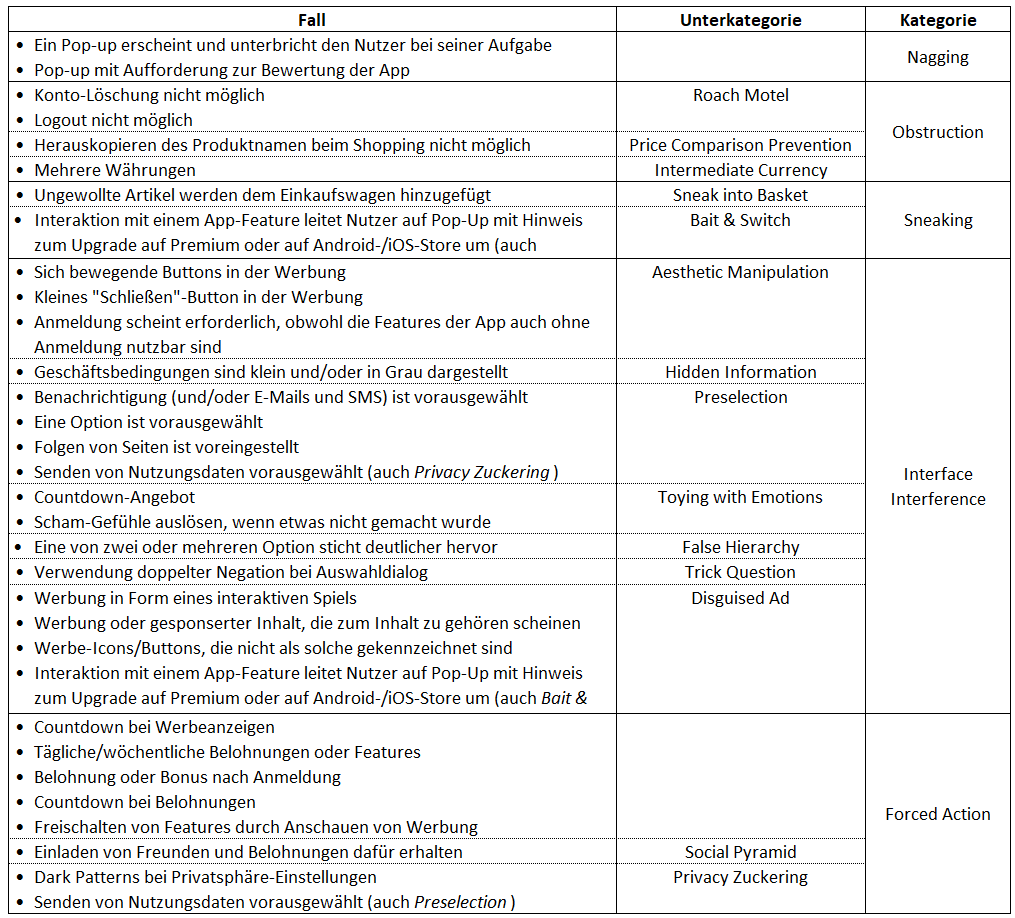
\includegraphics[scale=2.7]{dark_patterns_mobile_ui2}
\end{figure}

\subsection{Privacy Dark Patterns}
\label{sub:privacy_dark_patterns}
Es existieren sogenannte Privacy Design Strategien, die in der Entwicklungsphase iterativ zur Optimierung der Privatsphäre des Nutzers angewandt werden können. Das Konzept ist eine Erweiterung des Privacy by Design Prinzips, welches schon seit den 90ern als Grundlage dient, und sieht vor, dass Nutzern die Kontrolle über ihre eigenen Daten erleichtert wird \cite{boesch}. Acht Strategien wurden dafür definiert: \textit{Minimize}, \textit{Hide}, \textit{Separate}, \textit{Aggregate}, \textit{Inform}, \textit{Control}, \textit{Enforce}, \textit{Demonstrate}.\newline
Online-Dienste, die nicht die Interessen ihrer Nutzer berücksichtigen, wenden hingegen gewinnbringende Strategien an, um möglichst effizient persönliche Daten zu sammeln. Die Privatsphäre der Nutzer wird geschwächt, indem sie dazu gebracht werden, ihre persönlichen Daten mitzuteilen und Bedingungen zuzustimmen, die nicht ihren eigentlichen Interessen entsprechen. Diesbezüglich beschreiben Bösch et al. acht Strategien, die genau das Gegenteil der Privacy Design Strategien darstellen: 
\textit{Maximize}, \textit{Publish}, \textit{Centralize}, \textit{Preserve}, \textit{Obscure}, \textit{Deny}, \textit{Violate}, \textit{Fake}. Anhand dessen konnte das Team Privacy Dark Patterns erkennen und kategorisieren, die im Weiteren näher erläutert werden.

\subsubsection{Immortal Accounts}
\label{sssec:immortal_accounts}
Dem Nutzer wird es erschwert oder sogar unmöglich gemacht, sein Konto zu löschen. Zudem kann die Löschung vorgetäuscht werden, während in Wirklichkeit (einige) persönliche Daten behalten werden. Letztendlich können die Barrieren dazu führen, dass der Nutzer sich dagegen entscheidet, sein Konto zu löschen, um sich unnötige Mühen zu ersparen.\newline
Dieses Dark Pattern kann Grays et al. \hyperref[sssec:obstruction]{\textit{Obstruction}}-Kategorie zugeordnet werden.

\subsubsection{Hidden Legalese Stipulations}
\label{sssec:hidden_legalese_stipulations}
Geschäftsbedingungen sind oft zu lang gestaltet und schwer verständlich formuliert. Aufgrund dessen lesen viele Nutzer diese nicht, wodurch er angreifbar wird, wenn er den Bedingungen dennoch zustimmt. Denn es können Klauseln in den Geschäftsbedingungen versteckt sein und oftmals ohne Vorankündigung verändert werden.\newline
Dies stimmt mit Grays et al. Kategorie \hyperref[sssec:interface_interference]{\textit{Interface Interference}} überein.

\subsubsection{Bad Defaults}
\label{sssec:bad_defaults}
Standard-Optionen werden so gesetzt, dass der Nutzer dazu angeregt werden soll, seine persönlichen Informationen mit dem Service zu teilen. Die meisten Menschen haben keine Zeit, um alle Konfigurationen zur Privatsphäre durchzugehen und an seine Bedürfnisse anzupassen. Infolgedessen geben Nutzer oft mehr über sich preis, als sie beabsichtigen, wie Informationen über den Online-Status, Teile des Nutzerprofils oder Seitenbesuche. Dieses Dark Pattern wird meistens verwendet auf Web- und mobilen Applikationen, vor allem in Sozialen Netzwerken.\newline 
Grays et al. \hyperref[para:preselection]{\textit{Preselection}} (\textit{Interface Interference}) ist hiermit vergleichbar.

\subsubsection{Privacy Zuckering}
\label{sssec:privacy_zuckering2}
(siehe \hyperref[para:privacy_zuckering]{I.2.5.2})

\subsubsection{Address Book Leeching}
\label{sssec:address_book_leeching}
Der Nutzer wird nach Zugriffsrechten auf sein Adressbuch gefragt, damit er sich mit seinen Kontakten verbinden kann. Jedoch werden die Kontaktdaten intern gespeichert und für die Weiterverarbeitung genutzt, ohne dass der Nutzer darüber in Kenntnis gesetzt wird. Die Kontakte erhalten Einladungen oder Werbung, die oft im Namen des Nutzers versendet werden. Die Daten können auch genutzt werden, Profile zu erstellen und Individuen zu tracken.\newline
Dieses Dark Pattern hängt mit Brignulls \textit{Friend Spam} zusammen.

\subsubsection{Shadow User Profiles}
\label{sssec:shadow_user_profiles}
Daten über unregistrierte Personen können ohne ihre Zustimmung und ihr Wissen gesammelt und aufgezeichnet werden. Diese Informationen erhält der Dienstleister von importierten Adressbüchern registrierter Nutzer (z.B. via \textit{Address Book Leeching}), Metadaten oder Erwähnungen und können dazu genutzt werden, um Algorithmen zu verbessern, wie die Empfehlung von Kontakten oder Ad Targeting.

\subsection{Dark Game Design Patterns}
\label{sub:games}
Forscher im Bereich Game Design betonen häufig die Wichtigkeit von \textit{Player-centric Design}. Demzufolge ist ein Game Designer verpflichtet, ein unterhaltsames Spielerlebnis zu liefern und die Wünsche der Spieler möglichst zu berücksichtigen.\newline
Es kommt jedoch auch vor, dass Spieleentwickler eigene Interessen verfolgen und wenig Wert legen auf den Willen und die Bedürfnisse der Spieler. Zagal et al. definieren verschiedene Dark Patterns, die negative Erlebnisse beim Spieler erzeugen können \cite{zagal}.

\subsubsection{Temporal Dark Patterns}
\label{sssec:temporal_dark_patterns}
Sorgen dafür, dass Spieler mehr oder weniger Zeit als erwartet mit einem Spiel verbringen. Oft kann dabei das Gefühl entstehen, dass Spieler ihre Zeit verschwenden.

\paragraph{Grinding}
\label{para:grinding}
ist die Ausführung wiederholender, langwieriger Aufgaben durch den Spieler und kommt vor allem in MMORPG\footnote{\label{foot:8} MMORPG steht für das Videospiel-Genre \textit{Massively Multiplayer Online Role-Playing Game}, bei dem mehrere Spieler online miteinander interagieren können.} und Social Media Games\footnote{\label{foot:9} Social Media Games ist ein Typ von Videospielen, das über ein Soziales Netzwerk gespielt werden kann.} vor \cite{nakamura}. Es ist ein wohlbekanntes, jedoch umstrittenes Konzept für Gamer, wodurch der Spieler Fortschritt machen und Belohnungen erhalten kann. Allerdings hat diese Aktivität ein hohes Suchtpotential \cite{king}.\newline 
Vor allem Spieler, die sich mit anderen messen wollen, sind betroffen, da sie zur Erreichung ihrer Ziele anstreben müssen, besser zu werden. Für diejenigen, die sich dem Grinding verweigern, kann das Spielerlebnis eher beeinträchtigt werden. 

\paragraph{Playing by Appointment}
\label{para:playing_by_appointment}
verlangt vom Spieler, zu einem bestimmten, vom Spiel festgelegten Zeitpunkt, das Spiel wieder aufzunehmen. In einigen Fällen droht dem Spieler ansonsten der Verlust des Fortschritts, den er in einem Spiel gemacht hat.\newline
In \textit{FarmVille} zum Beispiel, einem beliebten Social Network Game, werden Pflanzen gesät, um Punkte und Ressourcen zu erhalten, und diese müssen zu einem bestimmten Zeitpunkt (nach genau 24 Stunden) geerntet werden, bevor sie auf Anhieb verwelken. Der Spieler wird also dazu verpflichtet, seinen Tagesablauf dementsprechend anzupassen.

\subsubsection{Monetary Dark Patterns}
\label{ssec:monetary_dark_patterns}
Spieler sollen dazu gebracht werden, mehr Geld auszugeben als erwartet oder erhofft. Kann zu Reuegefühlen, Verlust von Zeitgefühl und zu Geldverlust führen.\newline
Nicht zu verwechseln mit Glücks- oder Wettspielen.

\paragraph{Pay to Skip} 
\label{para:pay_to_skip}
ist ein Konzept, das zu Arcade-Zeiten der 80er Jahre vertraut war, in dem man zum Fortfahren des Spiels eine Münze in den Automaten werfen musste. Heutzutage tritt dieses Dark Pattern oft in Free-to-play Games\footnote{\label{foot:10} Free-to-play Games sind grundsätzlich kostenlos spielbar und beinhalten oft kostenpflichtige Inhalte oder Werbung.} und Social Media Games auf. Es sieht vor, dass Spieler Geld ausgeben, um in einem Spiel voranzukommen.\newline
Bei dem Augmented Reality Spiel \textit{Harry Potter: Wizards Unite} kann eine bestimmte Aktion nur mit einer Währung innerhalb des Spiels ausgeführt werden, und wenn diese aufgebraucht ist, muss man entweder ein sog. Gasthaus besuchen, oder (wenn kein Gasthaus in der Nähe ist) darauf warten, dass der Timer abgelaufen ist und der Spieler einen vom Spiel festgelegten Betrag der Währung erhält. Die Hauptfunktion des Spiels ist während dieser Wartezeit nicht verfügbar, somit ist das Weiterspielen unmöglich. Der Spieler kann diesen Timer mit Echtgeld überspringen.

\paragraph{Pre-Delivered Content}
\label{para:pre_delivered_content}
bedeutet, wenn trotz Erwerben eines Spiele-Exemplars bestimmte Inhalte oder Funktionen erst mit Zahlung einer Gebühr freigeschaltet werden müssen. Der Spieler bekommt dadurch das Gefühl, ein unvollständiges Spiel erworben zu haben.\newline
Die aktuellen Spiele der \textit{Tekken}-Serie bietet mehrere spielbare Charaktere an, von denen viele erst gegen eine Gebühr ausgewählt werden können. 

\paragraph{Monetized Rivalries} 
\label{para:monetized_rivalries}
wird auch als \textit{Pay to Win} bezeichnet und steht im Zusammenhang mit \textit{Grinding}. In manchen Spielen kommt es vor, dass das Ansammeln von In-Game Währungen so langsam voran geht, dass sich ein Spieler sehr lange mit Grinding beschäftigen muss, um die für das Weiterkommen notwendigen Gegenstände freischalten zu können.\newline
Ein Spieler kann sich, vor allem bei Wettkämpfen, durch Cheat Codes\footnote{\label{foot:11} Cheat Codes oder Cheats sind Einflussmöglichkeiten auf den Spielverlauf, die ursprünglich nicht vorgesehen sind und werden von Spielern verwendet, die ein Spiel zu ihren Gunsten manipulieren wollen.} oder schwer zu bekommende Gegenstände Vorteile gegenüber anderen Spielern verschaffen, indem er Echtgeld in eine In-Game Währung investiert. Somit können Top-Ränge und die damit verbundenen Bonusinhalte erreicht werden, wenn mit Echtgeld immer wieder Upgrades oder neueste Gegenstände erworben werden, während es weniger zahlungsfähigen Spielern unmöglich gemacht wird, eine Position in der Bestenliste zu erreichen.\newline
In dem Social Media Game \textit{Candy Crush Saga} ist es für den Spieler erforderlich, Geld im Spiel zu kaufen, um gegenüber seinen Facebook-Freunden konkurrenzfähig zu bleiben.  

\subsubsection{Social Capital-Based Dark Patterns}
\label{sssec:social_capital_based_dark_patterns}
Spieler erhalten starke Anreize, wie Boni und Vorteile im Spiel, wenn sie ihre Freunde und Familienmitglieder zum Spielen einladen.

\paragraph{Social Pyramid Schemes}
\label{para:social_pyramid_schemes}
macht Gebrauch von den Beziehungen des Spielers, bei dem dieser pro eingeladenem Freund Spiele-Vorteile bekommt. Oft werden bestimmte Funktionen erst freigeschaltet, wenn man eine bestimmte Anzahl an Freunden hinzugefügt hat.

\paragraph{Impersonation}
\label{para:impersonation}
wird vor allem in Social Network Games genutzt und ist vergleichbar mit Brignulls \textit{Friend Spam}. Hier werden die Namen aus der Kontaktliste des Spielers für Benachrichtigungen an ihn selbst verwendet. So erhält ein Spieler zum Beispiel eine Nachricht über ein Geschenk eines Freundes, obwohl dieser Freund eine solche Aktion gar nicht ausgeführt hat. Somit wird der Spieler dazu motiviert, das Spiel (weiter) zu spielen. Der Spieler kann sich dadurch auch verpflichtet fühlen, ein Geschenk zurück zu senden.

\subsection{Proxemische Interaktions-Systeme}
\label{sub:proxemische_interaktions-systeme}{}
Die Proxemik ist ein Forschungsgebiet, 
Der Begriff der \textit{Proxemik} wurde vom Anthropologen Edward T. Hall im Jahr 1960 vorgestellt und umfasst die Theorie über non-verbale Kommunikationswege, die erklärt, wie Menschen ihre Umgebung wahrnehmen und nutzen, um Kommunikationsziele zu erreichen \cite{communicationstudies}. Der Theorie zufolge ist die physische Distanz zu anderen abhängig davon, in welcher Beziehung die Kommunikationspartner zueinander stehen. S. Greenberg hat den Begriff der \textit{Proxemischen Interaktion} wie folgt definiert \cite{marquardt}:\newline 
\begin{quote}
\textit{[...] Diese Erwartungshaltung des Menschen kann gegenüber der Proxemik für Interaktionsdesign genutzt werden, um die Interaktion zwischen Mensch und [digitalen] Geräten in einer Ubicomp-Umgebung\footnote{\label{foot:1}Ubiquitous computing (Ubicomp) ist ein Konzept in der Softwaretechnik und Informatik, bei dem Computer jederzeit und überall eingesetzt werden können} zu beeinflussen. So wie die Menschen zunehmendes Engagement und Intimität erwarten, wenn sie auf andere zugehen, so sollten sie es auch als natürlich empfinden, dass die Konnektivität und Interaktionsmöglichkeiten zunehmen, wenn sie selbst und ihre Geräte sich in unmittelbarer Nähe zueinander befinden. Dies wird als Proxemische Interaktion bezeichnet.}
\end{quote}
Greenberg et al. erstellten eine Prognose, wie diese Technologie potentiell missbraucht werden könnte \cite{greenberg}. Nachfolgend wird diese zusammenfassend erläutert.

\subsubsection{The Captive Audience}
\label{sssec:the_captive_audience}
Eine Technologie wird im Raum strategisch platziert und nutzt die Gelegenheit der \glqq Gefangenschaft\grqq{} von Personen zu eigenen Zwecken aus, die an einem bestimmten Ort ein Ziel erreichen möchten, welches eine gewisse Zeit in Anspruch nimmt. So müssen Menschen beim Aufsuchen eines Ortes zur Durchführung einer Routine hinnehmen, dass das System eine unaufgeforderte und möglicherweise ungewollte Aktion ausführt.\newline
Beispiele umfassen unter anderem Spiegelflächen-Werbung in öffentlichen Toiletten \cite{youtube} und öffentliche Werbeflächen. Ein weiteres Beispiel ist ein Projekt der Werbeagentur BBDO und dem Sender Sky Go, die einen Prototypen entwickelten, das über hochfrequentige Vibrationen Audio-Werbung für Pendler abspielt, sobald diese ihren Kopf an das Zugfenster lehnen \cite{zugfenster_ad}.  

\subsubsection{The Attention Grabber}
\label{sssec:the_attention_grabber}
Ein strategisch in der Öffentlichkeit platziertes, proxemisch-sensibles System erzeugt Aufmerksamkeit, nachdem es ins Blickfeld einer vorbeilaufenden Person kommt. Es soll den Passanten in einen Kunden verwandeln.\newline
Proximity Marketing, wie Apples iBeacon oder Samsung Proximity, ist ein Beispiel dafür \cite{proximity_marketing} \cite{proximity_marketing2}. Hier werden Kunden in der Nähe via Smartphone-Benachrichtigung Informationen zugesendet, wie Produkt-Vorschläge oder Angebote.

\subsubsection{Bait and Switch}
\label{sssec:bait_and_switch2}
Das System lockt einen Betrachter mit begehrenswerten Angeboten oder interessanten Informationen, sobald dieser allerdings darauf aufmerksam wird und sich der Anzeige nähert, verändert sich die Werbung. Daraufhin kann ihm ein Angebot angezeigt werden, das im Bezug auf Preis und Qualität nicht seinen Erwartungen entspricht, weil das zuvor angezeigte Produkt nicht mehr verfügbar ist. Es kann auch zur Darstellung von unerwarteter Werbung genutzt werden. Genauso ist es möglich, den Passanten nach einer Registrierung bei einem ungewollten Service zu fragen, damit er die Interaktion fortführen kann, was mit eventuellen Sicherheitsrisiken verbunden ist.\newline
Amnesty International platzierte 2009 eine Werbung an einer Bushaltestelle, die mithilfe von Eye Tracking erkennen konnte, wann ein Wartender auf die Anzeige schaut und kurz darauf wurde das Bild verändert. Zunächst wurde ein Bild angezeigt, die Häusliche Gewalt darstellte, und sobald man hinsah, zeigte das Bild ein vermeintlich glückliches Pärchen. Dies sollte auf Häusliche Gewalt aufmerksam machen mit dem Slogan \glqq Es passiert, wenn niemand hinsieht.\grqq{} \cite{amnesty_international}
Ein anderes, aktuelles Beispiel ist Öffentliches WLAN, wie am Bahnhof oder in Flughäfen. Personen werden mit angeblicher kostenloser WLAN-Verbindung angeworben, jedoch stellt sich erst später heraus, dass der Service erst nach einer Registrierung nutzbar ist. Nach erfolgreicher Verbindung ist die Surfgeschwindigkeit dann allerdings zu langsam und der Nutzer zieht möglicherweise ein Upgrade auf ein Premium-Angebot mit einer schnelleren Surfgeschwindigkeit in Erwägung.

\subsubsection{Making Personal Information Public}
\label{sssec:making_personal_information_public}
Sobald eine Person einen bestimmten Bereich betritt, werden seine persönlichen Informationen öffentlich sichtbar gemacht. So können persönliche Informationen, wie Kalender-Einträge, Benachrichtigungen oder Direktnachrichten, auf Geräten in der Nähe angezeigt werden, z.B. auf öffentlichen \glqq Ambient Displays\grqq{}. Diese Systeme haben eigentlich die Absicht, hilfreich zu sein, jedoch können Außenstehende diese persönlichen Informationen einsehen.\newline
In 2009 wagte eine niederländische Werbeagentur eine Guerilla-Marketing Aktion an einer Bushaltestelle von Fitness First in Rotterdam: Ein Gewichtssensor wurde in einer Sitzbank eingebaut und zeigte das Gewicht einer Person auf einem öffentlichen Display an, sobald diese Platz nahm \cite{fitness_first}.

\subsubsection{We Never Forget}
\label{sssec:we_never_forget}
Ein System identifiziert proxemische Interaktionen, weil eine permanente, fortbestehende (und ungewollte) Beziehung besteht. Der Verlauf von vergangenen proxemischen Interaktionen wird gespeichert, welcher dazu verwendet werden kann, Verbindungen wiederherzustellen, einen Informationsaustausch durchzuführen, und/oder um vorherige Kontexte wiederherzustellen (z.B. die Anzeige der letzten angezeigten Informationen).\newline
Ein typisches Vorkommnis sind WiFi Hotspots, mit der sich mobile Geräte verbinden können. Möglicherweise möchten Nutzer es bei einer einmaligen Nutzung, und trotzdem kommt es zu einer erneuten, automatischen Verbindung mit dem Service. Dies kann auch die Sicherheit des Nutzers gefährden, wenn beispielsweise jemand ein gestohlenes Handy verwendet und die Anmeldedaten des (ehemaligen) Nutzers missbraucht.

\subsubsection{Disguised Data Collection}
\label{sssec:disguised_data_collection}
Zur Verfügung gestellte Informationen eines bestimmten Services wird missbraucht, um Nutzerprofile mit Informationen anzureichern, ohne dass der Nutzer seine Zustimmung abgibt. Systeme, die proxemische Beziehungen nachverfolgen können, haben somit Zugang zu zahlreichen Daten über das Verhalten seiner Nutzer. Diese Infos können von Marketing-Abteilungen potentiell dazu genutzt werden, um Personen zu orten und zu verfolgen und dadurch herauszufinden, wie effektiv Marketing-Aktionen sind. Diese Technologie kann möglich gemacht werden mit bspw. RFID-Chips, Rundfunk-Mobil-telefone und Smart Cards. Viele öffentliche Displays arbeiten bereits mit Computervision, um proxemische Interaktionen nachzuverfolgen, demnach können Bildaufnahmen analysiert und Personen dadurch identifiziert werden. Zudem können kostenlose WiFi-Dienste aufspüren, an welchem Standort beziehungsweise in welchem Geschäft sich eine Person befindet, indem die Signalstärke und die IP-Adresse des Geräts innerhalb eines Geschäfts gelesen wird.\newline
Kombiniert mit anderen Daten-Ansammlungen, z.B. dem proxemischen Interaktionsverlauf (\textit{We Never Forget}), kann ein noch ausführlicheres Profil erstellt werden.

\subsubsection{The Social Network of Proxemic Contacts or Unintended Relationships}
\label{sssec:the_social_network_of_proxemic_contacts}
Das System verfolgt die proxemischen Beziehungen des Nutzers zu anderen und konstruiert auf dessen Basis ein soziales Netzwerk. Dabei geht es davon aus, dass der Nutzer in einer sozialen Beziehung zu diesen Personen steht, auch wenn dies nicht der Fall ist.\newline
Mit den Daten könnten Marketer beispielsweise Zielgruppen durch demographische Merkmale erkennen. Die Techniken, die in \textit{Disguised Data Collection} beschrieben wurden, können auch dazu genutzt werden, soziale Beziehungen abzuschätzen, indem bspw. physische Distanz oder gemeinsame Interessen analysiert werden.

\subsubsection{The Milk Factor}
\label{sssec:the_milk_factor}
Ein proxemisches System zwingt eine Person, durch einen bestimmten Ort zu gehen oder diesen aufzusuchen, um einen Service zu erhalten.\newline
Ähnlich wie in Supermärkten, wo Produkte strategisch platziert sind, um die Sichtbarkeit von bestimmten, promoteten Gegenständen und somit Impulskäufe zu erhöhen, können proxemische Interaktionen dafür sorgen, dass in Zonen bestimmte Funktionalitäten unzugänglich sind, damit Menschen sich zu bestimmten Orten begeben.\newline
In Japan etwa gibt es Getränkeautomaten, die, wenn man weit weg steht, Werbebilder zeigen, angepasst an die aktuelle Jahreszeit, Temparatur und Tageszeit. Erst, wenn man sich dem Automaten nähert, kann man erkennen, welche Getränke angeboten werden. Demographische und Verkaufs-Daten werden ohne Einwilligung auf dem Firmenserver hochgeladen und für Analysen und zu Marketing-Zwecken verwendet.

\subsection{Home Robots}
\label{sub:home_robots}
Wie bei den Proxemischen Interaktionssystemen gesehen, beschränken sich Dark Patterns nicht nur auf Screen-basierte Technologien. Allmählich nimmt die Bedeutung von Ubicomp-Geräten zu, da sie zunehmend in das alltägliche Leben integriert werden. Home Robots sind eine smarte Technologie, zu denen der Mensch gleichzeitig eine emotionale Beziehung aufbauen kann. Die Nutzung birgt laut Lacey und Caudwell allerdins auch Risiken, die nachfolgend beschrieben werden \cite{lacey}.

\subsubsection{Illusion of user sovereignty}
Dem Nutzer wird durch das niedliche Aussehen des Roboters und dem \glqq Aufwachsen\grqq{} des Roboters in einer Familie ein Gefühl von digitaler Souveränität\footnote{\label{foot:12} Digitale Souveränität ist die Summe aller Fähigkeiten und Möglichkeiten von Individuen [...], ihre Rolle(n) in der digitalen Welt selbstständig, selbstbestimmt und sicher ausüben zu können. \cite{oeffentliche_it}}

\subsubsection{Short-term gains over long-term decisions/actions}
Dark Patterns stellen kurzfristige Gewinne über langfristige Entscheidungen oder Handlungen. Die Nutzung von Robotern kann sich langfristig auswirken auf die Entscheidungsfähigkeit des Nutzers und folglich die Gesundheit und das Wohlbefinden des Nutzers dauerhaft verschlechtern. Belohnungssysteme, die in die Interaktion mit dem Roboter eingebaut sind, setzen Dopamine frei und aufmerksamkeitserregende Methoden können für ständige Ablenkung sorgen, wodurch ein Sucht- oder Zwangsverhalten begünstigt wird. 

\subsubsection{Emotional data and data myopia}
Dark Patterns produzieren, manipulieren, verwalten und nutzen Emotionen, um beim Nutzer eine \textit{Data Myopia} bzw. Datenkurzsichtigkeit zu erzeugen. Das bedeutet, dass der Nutzer zugunsten von kurzzeitigen Empfindungen davon abgelenkt wird, darauf Acht zu geben, seine privaten Daten zu schützen.\newline
Home Robots bestehen auf die Sammlung und Verarbeitung persönlicher Daten, unter dem Vorwand, diese für die Optimierung der User Experience zu nutzen. Dabei werden viele persönliche Daten aufgezeichnet, ohne dass der Nutzer das mitbekommt. Möchte der Nutzer auf die Datenerhebung verzichten, Änderungen an den Datenschutzeinstellungen vornehmen oder bei Änderungen der Datenschutzrichtlinie auf dem aktuellsten Stand bleiben, wird dem Nutzer dies unnötig erschwert.\newline
Greenbergs et al. \hyperref[sssec:we_never_forget]{\textit{We Never Forget}} und Grays et al. \hyperref[subpara:toying_with_emotions]{\textit{Toying with Emotions}} stehen hiermit im Zusammenhang: Der Roboter ist so designt, dass der Nutzer ihm gegenüber eine starke Zuneigung, Bindung und Beschützerinstinkte entwickelt, den Nutzer jedoch gleichzeitig dazu zu verleitet, während der Interaktion ungewollt seine persönlichen Daten preiszugeben. Dadurch, dass Home Robots sich in der häuslichen Umgebung befinden, erfahren sie eine Menge über das Privatleben des Nutzers. Datengetriebene Unternehmen können von diesen emotionalen Daten Gebrauch machen und davon profitieren.

\newpage

\section{Schluss}
\label{sec:schluss}

\subsection{Ausblick \& Fazit}
\label{sub:ausblick}
Das Themenfeld der Dark Patterns umfasst viele Bereiche des alltäglichen Lebens und wird auch in Zukunft noch Relevanz haben. Einige Nutzungskontexte wurden bereits in wissenschaftlichen Arbeiten behandelt, jedoch besteht weiterhin Forschungs- sowie Aufklärungsbedarf. 
Wie bereits Geronimo et al. anhand von Tests feststellen konnte, dass Nutzer Dark Patterns bei mobilen Anwendungen oft nicht wahrnehmen (\textit{DP-blindness}), kann dies auch in anderen Anwendungen erforscht werden \cite{geronimo}. Nicht nur das Ergebnis dieses Experiments ist ein Hinweis darauf, dass Menschen auf Dark Patterns und die Schäden, die es anrichten kann, aufmerksam gemacht werden sollten. Auch der Erfolg der Unternehmen bei der Anwendung solcher Taktiken ist ein Indiz dafür.\newline\newline
Es existiert eine Plattform, die dabei helfen soll, gesunde Mobile Games zu finden \cite{dp_games}. Jeder registrierte Nutzer kann dazu Spiele bewerten und beurteilen, ob ein Spiel Dark Patterns beinhaltet.\newline
Vielversprechend ist auch das \textit{Dark Pattern Detection Project}, das Ende 2020 von einem interdisziplinären Team aus Informatiker und Rechtswissenschaftler ins Leben gerufen wurde und u.a. vom Bundesministerium der Justiz und für Verbraucherschutz gefördert wird \cite{dapde}. Ihr Ziel ist es, sowohl eine Open-Source App für Verbraucher zu entwickeln, die automatisch Dark Patterns erkennt, als auch rechtliche Regulierungsmöglichkeiten darzulegen.\newline
Um rechtlich gegen Dark Patterns vorgehen zu können, sollten Dark Patterns ethisch hinterfragt werden und auf Basis dessen klare Regulierungen dafür geschaffen werden. In den USA wurde laut dem Dokumentationsfilm \textit{The Social Dilemma} bereits eine Ethikgruppe namens \textit{DETOUR} (Deceptive Experiences To Online Users Reduction) Act gegründet, die sich in einem Gesetzesentwurf für den Verbot von solchen Plattformen ausgesprochen hat \cite{the_social_dilemma}.\newline
Abschließend sollte zudem in Hochschulen und bei Ausbildungen mit MCI- oder UX-Design-Schwerpunkt Ethik im Design gelehrt werden. Bei der Erarbeitung von Gestaltungslösungen sollten moralische Werte ebenfalls eine deutlich größere Rolle spielen. Unter anderem setzen Werte-zentrierte Methoden ihren Fokus auf ethische Aspekte, wie das \textit{Value-centered Design} (VSD)\footnote{\label{foot:13}Value-sensitive Design bezeichnet eine theoretisch fundierte Herangehensweise an den Entwurf von Technologie, die die menschlichen Werte in einer prinzipienfesten und umfassenden Weise während des gesamten Entwurfsprozesses berücksichtigt. \cite{gray}}, \textit{Values at Play}\footnote{\label{foot:14}Values at Play untersucht, wie Designer bewusster mit der Art und Weise umgehen können, wie sie menschliche Werte in ihre spielbasierten Systeme integrieren.} oder \textit{Value Levers}\footnote{\label{foot:15}Value Levels wurden als Mittel vorgeschlagen, um wertebezogene Einsichten mit Design-Handlungen zu verbinden.}.   


\newpage


\printbibliography

%\bibliography{Referenzen}

%\bibliographystyle{natdin}
	%\bibliography{references} % expects file "references.bib"
	%\addcontentsline{toc}{section}{References}
\end{document}